\documentclass[12pt, letterpaper]{article}  % change to >11 pt if you like, and change article with report
\usepackage[letterpaper, top=3.71cm, bottom=3.20cm, left=2.86cm, right=2.86cm]{geometry}
\usepackage[utf8]{inputenc}
\usepackage{natbib}
\usepackage{graphicx}
\usepackage{color}
\usepackage{subfig}
\usepackage{float}
\usepackage{hyperref}

\title{\vspace{-2cm}\textbf{Mobile and cyber-physical systems project specification}}
\author{\small{\textit{Dalla Noce Niko, Ristori Alessandro}.} \\ % put your full name here
        \small{Master Degree in Computer science.}\\ \small{{n.dallanoce@studenti.unipi.it, a.ristori5@studenti.unipi.it}.} \\  % put your Master Degree here
        \small{Mobile and cyber-physical systems, Academic Year: 2020/2021} \\
        \small{Date: 31/03/2021} \\
        %\small{Type of project: \textbf{A}}
        \small{Team 8}
}

\renewcommand\refname{} %remove this line to automatically show the bibliography header

\begin{document}

\nocite{*}  % comment this line to list only the articles you really cite
\date{}
\maketitle
\begin{center}
    
\includegraphics[width=0.2\textwidth]{images/unipi.png}\\
    \vspace{0.5cm}
\end{center}
\begin{abstract}
The document presents the problem we wish to address, a possible use case with the specifications necessary for the implementation of the project; there will also be a short paragraph in which we will talk about how we intend to carry out our idea.
%Il documento presenta il problema che desideriamo affrontare, un possibile caso d'uso con le specifiche necessarie all'implementazione del progetto; sarà presente anche un breve paragrafo nel quale parleremo di come abbiamo intenzione di portare avanti la nostra idea.
\end{abstract}
%\include{Sections/abstract}
\newpage
\section{Problem description}\label{sec:prob_desc}
The current HACCP regulations\footnote{\url{https://www.haccproma.it/it/conservazione-degli-alimenti-le-giuste-temperature}} regarding the preservation of foodstuffs impose on every retailer the obligation to keep updated a daily register containing the temperatures of the cold rooms. In case of non-compliance, the merchant had to pay a very substantial penalty.
\vspace{3mm}

It is certainly convenient for our customer to automatically know various information on the refrigerators' state (temperature, humidity, etc.) without the need to personally check their state; moreover, having this information always at hand is necessary in an increasingly smart world where everything is accessible via smartphone.
\vspace{3mm}

For this purpose we want to introduce \textbf{S.E.B.} that stands for Smart Environment Bot, as a valid solution both to the individual merchant and companies that need to keep up to date on the status of their cold rooms and, consequently, on their products that could end up in bad condition if something could malfunction.

\section{Use cases}
As we mentioned in the \textbf{\nameref{sec:prob_desc}} paragraph, our project aims to provide an efficient and fast solution for storing foodstuffs in cold stores by applying iot and smart elements in harmony: to do this we will use sensors to detect the temperature and humidity of the individual refrigerators; such data will be saved at the end of each time window decided by the user (which can vary upon request) on a database that will make the data available to the bot to whom the users will interface by issuing specific commands.
\vspace{3mm}

A fundamental point of our work is to give customers the opportunity to always be updated on the status of their refrigerators; in this regard, users can set a temperature limit beyond which the bot will send an alert in the chat: this allows for faster management of any malfunctions.
Furthermore, the bot will make it possible to obtain many informations such as the daily average temperature/humidity or the latest measurements made, so customers can always stay up to date on the status of their refrigerators.
\vspace{3mm}

Finally, each user will always be able to know the parameters of their sensors through a simple command and modify them as they wish to adapt them to their needs.
\newpage

\section{Requirements}\label{sec:requirements}
We'll use the following software/hardware platforms:
\begin{itemize}
    \item \textbf{Hardware} side:
    \begin{itemize}
        \item \textbf{Raspberry Pi 4 Model B} for sensor installation and to start the detection by running \textit{temperature.py};
        \item \textbf{DHT22 AM2302 AZDelivery} sensors for temperature and humidity detection.
    \end{itemize}
    \begin{figure}[H]%
        \centering
        \subfloat[Raspberry Pi 4 Model B]{{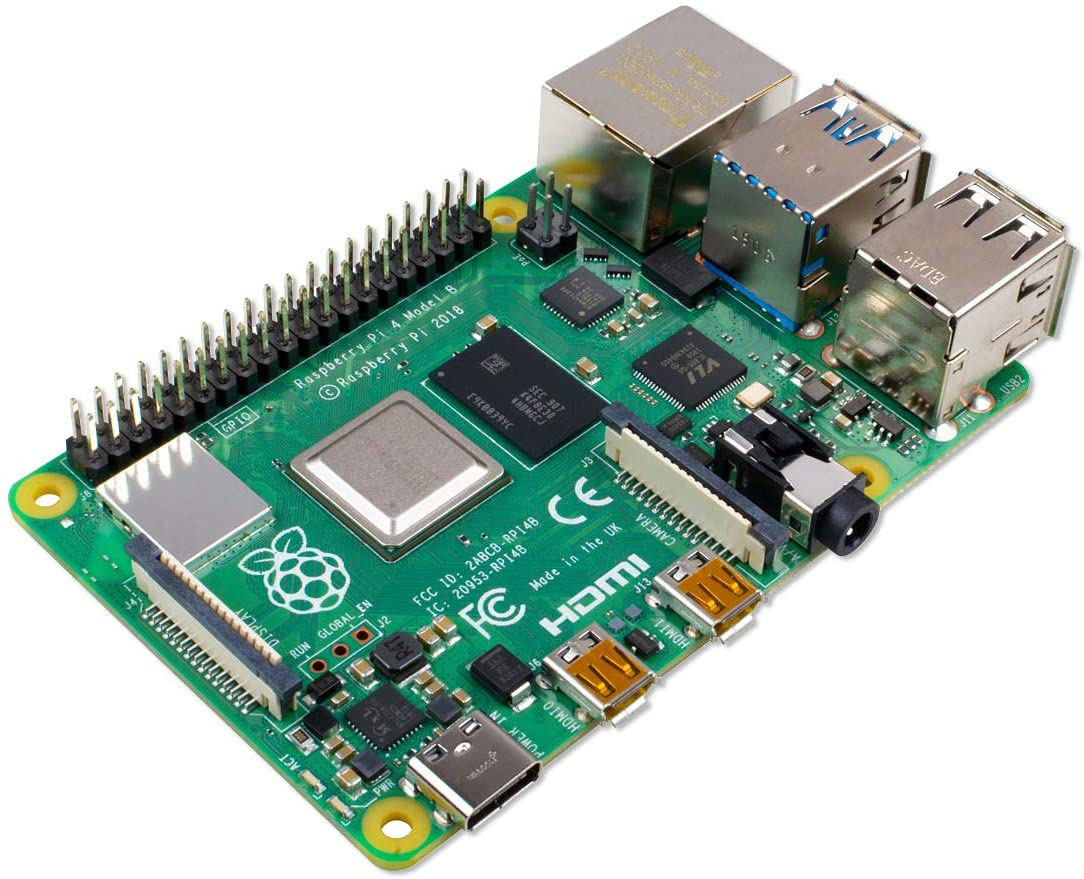
\includegraphics[width=0.31\linewidth]{images/Raspberry.png}}}%
        \hspace{10mm}
        \subfloat[AZDelivery DHT22 AM2302]{{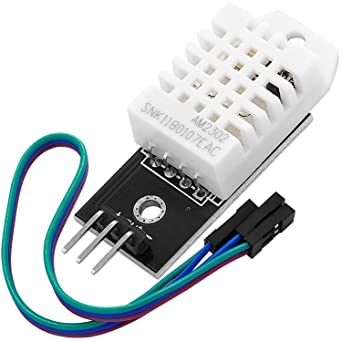
\includegraphics[width=0.2\linewidth]{images/Sensor.png}}}%
        %\hfill
        %\caption{Il problema del commesso viaggiatore, immagine trovata dal web}
        %\caption{Rappresentazione degli archi del grafo basato sul sudoku}
        %\caption{Articoli per anno contenenti "Genetic Algorithm", fonte dei dati: Google Scholar}
        \caption{The Rapsberry and sensors used in the project.}
        \label{fig:hardware}%
    \end{figure}
    \item \textbf{Software} side:
    \begin{itemize}
        \item \textbf{HiveMQ Cloud} for the MQTT broker;
        \item \textbf{MongoDB Atlas} to store the samples provided by the sensors and informations about our customers;
        \item \textbf{Telegram bot} to which the users will talk and ask for data by issuing commands;
        \item \textbf{Heroku} to host and execute both the Telegram bot and our server;
    \end{itemize}
    \begin{figure}[H]%
        \centering
        \subfloat[HiveMQ]{{
\includegraphics[width=0.20\linewidth]{images/hivemq.png}}}%
        \hspace{8mm}
        \subfloat[Mongodb]{{
\includegraphics[width=0.20\linewidth]{images/mongodb.png}}}%
        \hspace{8mm}
        \subfloat[Telegram]{{
\includegraphics[width=0.20\linewidth]{images/telegram.png}}}%
        \hspace{8mm}
        \subfloat[Heroku]{{
\includegraphics[width=0.20\linewidth]{images/heroku.png}}}%
        %\hfill
        %\caption{Il problema del commesso viaggiatore, immagine trovata dal web}
        %\caption{Rappresentazione degli archi del grafo basato sul sudoku}
        %\caption{Articoli per anno contenenti "Genetic Algorithm", fonte dei dati: Google Scholar}
        \caption{All the platforms we used to store/run our project.}
        \label{fig:software}%
    \end{figure}
\end{itemize}

Raspberry runs Raspberry Pi Os 32-bit (Release 10) with Python 3.7; for the detection of sensor data we used the Python library called adafruit\_dht.\vspace{3mm}

The Telegram bot was developed on Python 3.8, using the python-telegram-bot library, which communicates with MongoDB Atlas using pymongo.
\vspace{3mm}

The server was developed in Java (JDK 16) and has the aim of receiving messages from the MQTT broker, saving them in the database and eventually sending the alerts. The server interfaces with HiveMQ using the HiveMQ MQTT Client library, available at the following link \url{https://github.com/hivemq/hivemq-mqtt-client}. 

The database is managed through the official MongoDB library, available at the following address: \url{https://mongodb.github.io/mongo-java-driver/}. Finally, the alerts are sent to the Telegram bot using the Java Telegram Bot API library, hosted on GitHub at \url{https://github.com/pengrad/java-telegram-bot-api}.
\vspace{3mm}

The code written by us is available entirely on GitHub to the following link (server and bot are in the description provided by the README.md): \url{https://github.com/nikodallanoce/MCPS}.

\section{Solution description}

\subsection{Raspberry}
DHT22 sensors are installed on the Raspberry, for temperature and humidity monitoring. Each customer can buy one or more Raspberry and consequently will own several sensors; each sensor publishes its measurements in a topic which is in this format: "\textbf{customer} / CustomerName / Place / ThingToMesure" (for example "customer / Customer1 / warehouse / fridge1"), at each time interval defined in the database and it can be modified at any time.
\vspace{3mm}

Each sensor connects to the MQTT Broker via username and password due to the fact that HiveMQ Cloud only accept this kind of communications and to increase the system security as well, so it uses the 8883 port. Also, each sensor has a subscription to the topic "\textbf{communication}/ CustomerName/ Place/ ThingToMeasure", through which it receives informations from the server regarding how often send data. Once started, the Raspberry cannot go to sleep because this function has not been implemented on the Raspberry OS. However, we wanted to minimize the use of the processor in order not to waste energy unnecessarily, so we decided to associate a thread with each sensor, which goes into sleep after it has received information from the server regarding how often it sends the surveys. Going into detail, each thread performs the following operations, in order:
\begin{enumerate}
    \item Publishes a detection in a topic;
    \item Receives an indication about how often it should send the data from the server;
    \item Sleeps.
\end{enumerate}

In details, a thread handles the operations of two MQTT clients, a publisher and a subscriber. The first operates with Quality of Service equal to one, while the second with QoS equal to 2.

\subsection{Server}
The server connects the sensors to the database and eventually sends the alert messages and is subscribed to the topic "\#"\footnote{The simbol "\#" indicates the subscription to each topic available in the MQTT broker.} with Quality of Service equal to 2. This choice adds overhead in the communications, but in this way it is not necessary to control the duplicates when the messages arrives into the server. Futhermore, both the Java server and the MQTT broker, in this scenario, are designed to work always on and plugged to the power supply.
\vspace{3mm}

There are two queues on the server, one called "topicPayload" and the other called "alerts". When the broker sends a message to the server, the topic and payload associated with the message are inserted into the first queue and then a thread takes care of retrieving each element of this list and inserts the data of the sensor detections into the database. In the event that a detection exceeds the threshold associated with a specific topic, the alert message is inserted on the "alerts" queue. This queue is managed by another thread, which takes care of sending all alerts to their respective customers that will receive the message from the bot in the Telegram chat. In order to keep a history of the alerts, these are then inserted into a collection of the database called "Alerts".
\vspace{3mm}

Finally, for each message received by the broker other than the "communication" type, the server communicates to the sensor how long it has to wait before sending a new survey, through a publish in the topic "communication/ Topic", where "Topic" is the topic in which the sensor executes the publish.

\subsection{Database}
By looking at schema in figure \ref{fig:dbcollections} is possible to have a general idea over our non-relational database works; the database was built adapting the relational database we had in mind.
\begin{figure}[H]%
    \centering
    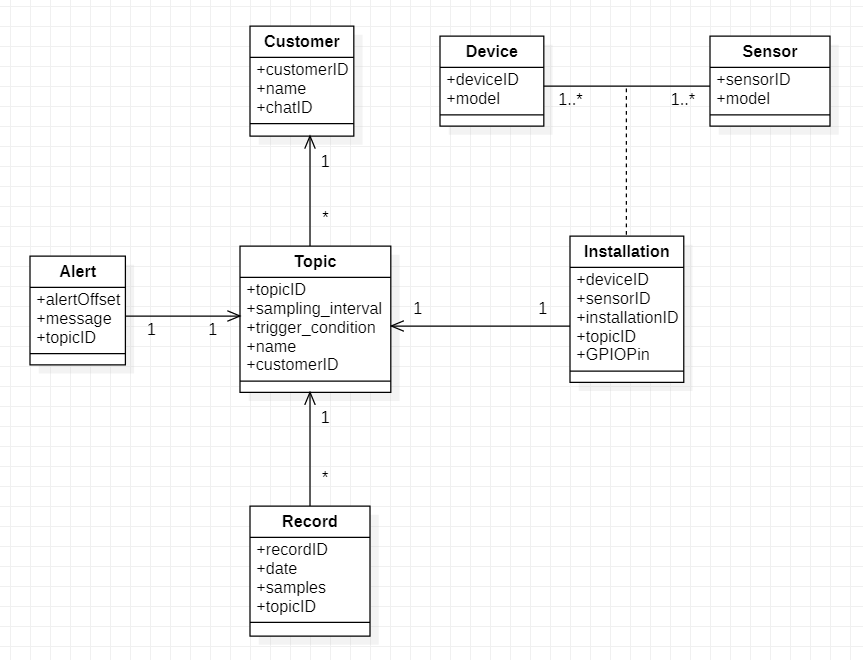
\includegraphics[width=0.9\linewidth]{images/collections.png}
    \caption{The UML schema of our software.}
    \label{fig:dbcollections}
\end{figure}
Below we can find a detailed description of the many collections and their fields that compose our database (the ID fields aren't listed since they are set automatically by Monogdb):
\begin{itemize}\label{list:collections}
    \item \textbf{Customers}
    \begin{itemize}
        \item \textit{name}, customer's name, can be different from the username on telegram;
        \item \textit{chatID}, the telegram chat ID for a user or group.
    \end{itemize}
    \item \textbf{Topics}
    \begin{itemize}
        \item \textit{sampling\_interval}, the interval beetween one sample and the next one;
        \item \textit{trigger\_condition}, the threshold at which the bot sends an alert if the temperature is higher than the value contained in this field;
        \item \textit{name}, it follows the rule CustomerName/topic/subtopic/....
    \end{itemize}
    \item \textbf{Sensors}
    \begin{itemize}
        \item \textit{model}, the sensor's model, in our case a DHT22.
    \end{itemize}
    \item \textbf{Devices}
    \begin{itemize}
        \item \textit{model}, the device's model, in our case a Raspeberry Pi 4 model B.
    \end{itemize}
    \item \textbf{Alerts}
    \begin{itemize}
        \item \textit{alertOffset}, the interval that the server waits before sending another alert.
        \item \textit{message}, an array with the messages the server sends when an alert is sent. It's the alert history for a topic.
    \end{itemize}
    \item \textbf{Records}
    \begin{itemize}
        \item \textit{date}, the date of the temperature and humidity detection;
        \item \textit{samples}, two arrays, one for the daily temperature and one for the daily humidity, each element of those arrays contains a value and a timestamp.
    \end{itemize}
\end{itemize}
\vspace{3mm}

Let's focus more on the Records collection, we insert a new document daily (by topic), each containing, in addition to the ID and the reference date, two arrays to record temperatures and humidity. This solution was conceived as a meeting point between having a new document for each sensor detection and having a single document containing all the detections.

\subsection{Telegram Bot}
As we mentioned in the \textbf{\nameref{sec:requirements}} paragraph, most of the work is done through the use of the python-telegram-bot library which provides a high-level api for the management of the bot's commands, we also use the pymongo library for the querying the database on monogdb atlas. We have decided to provide the user the ability to send the following commands:
\begin{itemize}
    \item \textbf{Utils}:
    \begin{itemize}
        \item \textit{/help} - Shows a list of all possible commands;
        \item \textit{/user} - Shows informations about the user;
        \item \textit{/topics topic} - Shows every topic the user is subscribed to (if no argument is passed).
    \end{itemize}
    \item \textbf{Modify Parameters}:
    \begin{itemize}
        \item \textit{/changeoffset topic offset} - Changes the sampling interval of the desired topic (to which the user is subscribed to)
        \item \textit{/changetrigger topic trigger} - Changes the trigger condition of the desired topic (to which the user is subscribed to)
        \item \textit{/setalert topic offset} - Changes the alert offset of the desired topic (to which the user is  subscribed to)
    \end{itemize}
    \item \textbf{Return Records:}
    \begin{itemize}
        \item \textit{/avgtemp topic year-month-day} - Gives the average temperature of the current day if no argument is passed
        \item\textit{/avghum topic year-month-day} - Gives the average humidity of the current day if no argument is passed
        \item \textit{/lasttemp topic year-month-day} - Returns the last recorded temperature of the current day if no argument is passed
        \item \textit{/lasthum topic year-month-day} - Returns the last recorded humidity of the current day if no argument is passed
    \end{itemize}
\end{itemize}
To communicate with the bot it is only necessary entering the command and then insert the various arguments for the desired operation. If the command entered is wrong an error message will be returned. In case we don't remember some commands, you can type "/" in the chat, which will show us all of them.
\begin{figure}[H]%
    \centering
    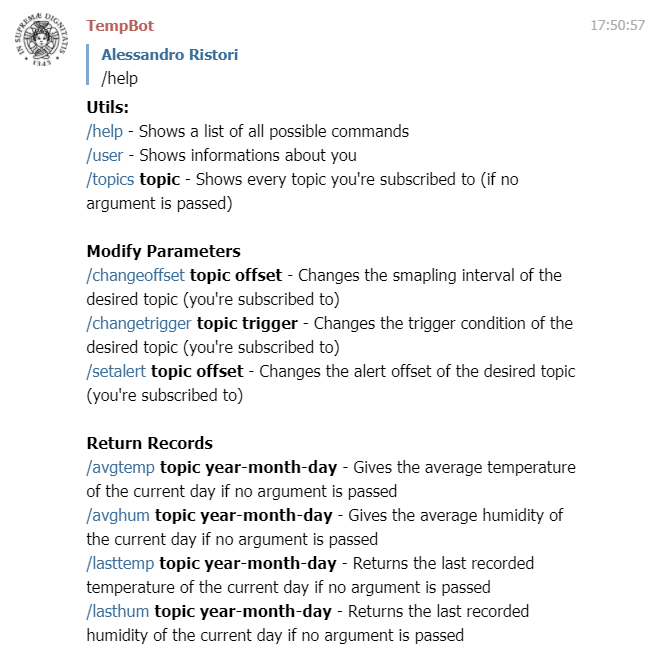
\includegraphics[width=0.59\linewidth]{images/botcommand.png}
    \caption{An example of the bot answering to a command, in this case \textit{/help}}
    \label{fig:botcommand}
\end{figure}
The bot is hosted on Heroku, so it's always available every time someone needs to issue it commands, it can be reached to the following link \url{https://t.me/MCPSbot} if you're in a browser or you can search it by name on Telegram.

\section{Planned demo and future work}
We will show  our project taking into account the scalability factor and the architecture behind our software, the aim of the presentation is to give our colleagues an overwiew of what we have done and how we did it by showing them a quick demo of our project. 
\vspace{3mm}

During the presentation, after the necessary preparations and having explained the architecture behind our project, we will show how the data is retrieved and collected and how an alert message is sent to the chat. Later, we'll open a predisposed telegram chat to interface the bot with the aim to execute the many available commands: in particular we will show how to view the topics we are subscribed to and how to retrieve data, like the average temperatures and the latest recorded surveys.\vspace{3mm}

We are extremely interested in expanding our work with the possibility of sending sms in parallel with the bot, in order to make everything more accessible even to the older groups of customers: In addition we could create an app that can give greater management concerning the sensors and a better data display, for example introducing graphs. In addition, the structure of the software, including the database, gives an high flexibility of application domains, ranging from home to business. In addition, we could integrate voice assistants, such as Amazon Alexa and Google Assistant, asking them directly the data that we want to know.
%\input{Sections/method}
%\input{Sections/experiments}
%\input{Sections/conclusion}
%\input{Sections/references}

\end{document}
